\subsection{Caracterización de las palabras identificadas como contrastivas}


\begin{frame}[t]\frametitle{Pipeline}
    
\begin{figure}
  \centering
  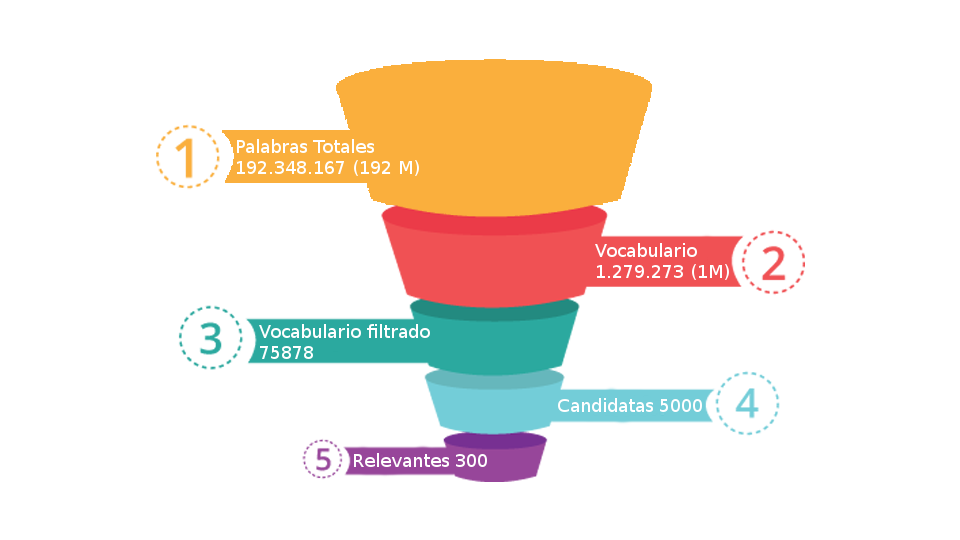
\includegraphics[width=0.95\textwidth]{../src/images/presentacion/embudo.png}
  \label{fig:embudo}
\end{figure}

\end{frame}

\begin{frame}[c]\frametitle{Validación lingüística}

  \textbf{Trabajo realizado por la Academia Argentina de Letras (AAL):}
   
  
    \begin{itemize}

      \label{it:caracterizacionLinguistica}
      
      \item \textbf{Coloquialismos o vulgarismos}

      % \blockquote[Córdoba]{Perdon pero tenes que ser muy \textbf{culiado/a} para ir a mc y pedirte una ensalada}


      \blockquote[Mendoza]{Q \textbf{chombi} hacer un chiste y q la otra persona no se ría o no lo entienda}
      
      \blockquote[Neuquén]{Que \textbf{carnasas} poniendole rosas rojas a toda la ropa, para mi queda horrible sorry}

      %   \blockquote[Chaco]{Teres, \textbf{pororós} y pelis con Carlita y Flor}

      % \blockquote[San Juan]{Ver un negro \textbf{chuño} con musculosa y gorro.. se ve que el tipo no quería pasar ni frío ni calor.}

      % \blockquote[Formosa]{Tenía la re expectativa para este sábado y al final \textbf{trancó} todo }
     
       \item \textbf{Indigenismos}

      \blockquote[Formosa]{Te regalo ser \textbf{mitaí} y ir a jurar la bandera con el guardapolvo caliente ese y la corbata que te ahorca todo (Del guaraní mitaí “pequeño”)}

      \blockquote[Corrientes]{\textbf{Angá} mi negrito, esta triste (Del guaraní angá aprox. “pobre”)}

     
     
      % \item \textbf{Gentilicios}

      % \textbf{Casildense} (de Casilda), \textbf{concordiense} (de Concordia) y \textbf{obereño} (de Oberá).
      % }
     

\end{itemize}

   
   
% \item \textbf{Voces no marcadas en registro, que aluden a una realidad local}

%   \blockquote[San Juan]{Quiero a alguien que me diga vamos a comer \textbf{piadinas}, un pancho, un chori, una hamburguesa lo que sea y soy feliz}

%   \blockquote[Misiones]{\textbf{Tareferos} que reclamaban asistencia interzafra en Posadas estarían preparando una protesta para hoy en la Fiesta del Inmigrante en Oberá.}

%   \blockquote[Jujuy]{Me encantan los bohemios anti sistema que usan vans. Es como que seas ecologista y uses un cuaderno hecho con media \textbf{yunga}.}

\end{frame}

\begin{frame}[c]\frametitle{Más resultados}
    
\only<1->{}
\begin{itemize}
  
  
  \only<1>{
  \item \textbf{Leísmo}

  \blockquote[Misiones]{No te olvides de \textbf{saludarle} a tu suegro hoy}

  \blockquote[Misiones]{Vine a \textbf{visitarle} a mis primas y estan re colgadas, para eso me quedaba en mi casa no maaa }

  \blockquote[Formosa]{A \textbf{esperarle} a nahuel, que traiga los teresss }

  }
% \item \textbf{Fusiones y acrónimos que pueden señalar pronunciación o alta frecuencia de uso}

%   \blockquote[Buenos Aires]{Los sueños de la siesta me dejan \textbf{patra} }

%   \blockquote[Córdoba]{Si mañana me dice q no, voy sola, necesito ver esa pelicula en el cine siosi}

% % \item \textbf{Voces consideradas generales pero que, al aparecer en la lista, permitieron verificar su contrastividad en frecuencia de uso al menos con respecto a España}
%   % Ejemplos: \textbf{pavada}, \textbf{distrital} y \textbf{cariño}.
\only<2>{
  
  \item \textbf{Voces sospechadas generales pero con acepción local diferente}

  % \blockquote[Mendoza]{Mañana que alguien \textbf{atine} con parque y porrones}

  \blockquote[San Juan]{\textbf{Mansas} ganas de sentarme a tomar un te con semitas}

  % \blockquote[Tierra del Fuego]{\textbf{Habilítenme} una nueva espaldaa}

  \blockquote[San Juan]{sigo \textbf{asada} por cosas que han pasado hace como dos dias, que falla (Mendoza) / Que \textbf{asada} estoy, tengo la cabeza echa un lío}
}

\only<3>{
  

\item \textbf{Voces con una morfología propia de una región}

Ejemplo: terminación azo/aza con base adjetiva.

  % \blockquote[San Juan]{Creo que va a estar \textbf{malazo} lo de esta noche } 

  \blockquote[Córdoba]{Esta \textbf{locaza} esa mina para hacer eso}
}
\end{itemize}

\end{frame}
\begin{frame}[c]\frametitle{Más resultados}

\only<1->{}    
\begin{itemize}

\only<1>{
\item \textbf{Formas verbales coloquiales con sustantivos o adjetivos como base}

  \blockquote[Neuquén]{Me calma mucho \textbf{mimosear} a mi perro }

  % \blockquote[Buenos Aires]{Me vine a acostar y ya me dicen que parezco de 80 años ME CHUPA UN HUEVO LO QUE PIENSEN, DEJENME \textbf{ABUELEAR} }

  \blockquote[Tierra del Fuego]{Estaría bueno que ari venga aunque sea a saludarme y que no se quede todo el tiempo \textbf{pollereando}.}

  
}

\only<2>{
\item \textbf{Vesres}: Creación de palabras por inversión de sílabas que se usa jergalmente o con fines humorísticos.

  \blockquote[Corrientes]{Estoy en lo de villa mateando con él y jimmy. Pinta \textbf{sogui} abundante más tarde dijeron }

  \blockquote[Chaco]{Uhhh me acuerdo si no habré saltado el muro del aguapey par colarme a los \textbf{cequin}. (cequín “fiesta de quince”)}
}

\only<3>{
\item \textbf{Intejercciones}

  \blockquote[Formosa]{\textbf{Aijué}, encima me decís vieja, re que no pinta esto facundo jaja ya te dije como es la onda, fin }

  \blockquote[Formosa]{\textbf{Ains}, una mujer hablando de fútbol.}

  \blockquote[Corrientes]{Al fin una buena: hora libreeee! \textbf{Yirr} }
% \end{itemize}
}
\end{itemize}
\end{frame}


\subsection{Validación estadística}

\begin{frame}[c]\frametitle{Problema desde el punto de vista estadístico}

  Utilizar tests estadísticos para validar los resultados.
  \medskip

  \begin{block}{Hipótesis nula: $H_0$}
    La palabra tienen un uso homogéneo en las distintas regiones de la Argentina, es decir que la frecuencia de ocurrencias de cada palabra debería ser similar independientemente de la región.
  \end{block}
\end{frame}



\begin{frame}[c]\frametitle{Test t de Welch}

   El test de Welch nos provee un valor de probabilidad para rechazar la hipótesis nula: las medias de las dos distribuciones son iguales.

   
       Las suposiciones del test 
        \begin{enumerate}
            \item Textos son estadísticamente independientes 
            \item La media de las frecuencias proviene de una distribución normal
        \end{enumerate}
  
       \begin{block}{Metodología}
              Agrupamos todos los tuits de cada usuario representando un texto.
              % \footnote{Notar que la suposición de independencia es más débil.}
        \begin{description}
            \item[Corpus S] Todos los textos sobre la región que cubre más del 80\% de las ocurrencias
            \item[Corpus T] Los textos creados por usuarios del resto de las provincias
        \end{description}

        \end{block}
\end{frame}


\begin{frame}[c]\frametitle{Resultados test t de Welch}

  \begin{enumerate}
    \alert<1>
    {
    \item Para cada métrica $I,I_W,I_P$  variamos los subconjuntos de palabras de acuerdo al listado ordenado según estas.
    }
    
    \alert<2>
    {
    \item Calculamos la tasa de rechazo de la hipótesis nula, definida por:
    \begin{equation}
      \text{Tasa de rechazo(tests)} = \frac{\# \{t:tests \mid p \text{-}valor(t) < 0.05\}}{\#tests} 
    \end{equation}
    } 
  \end{enumerate}

  \begin{figure}
  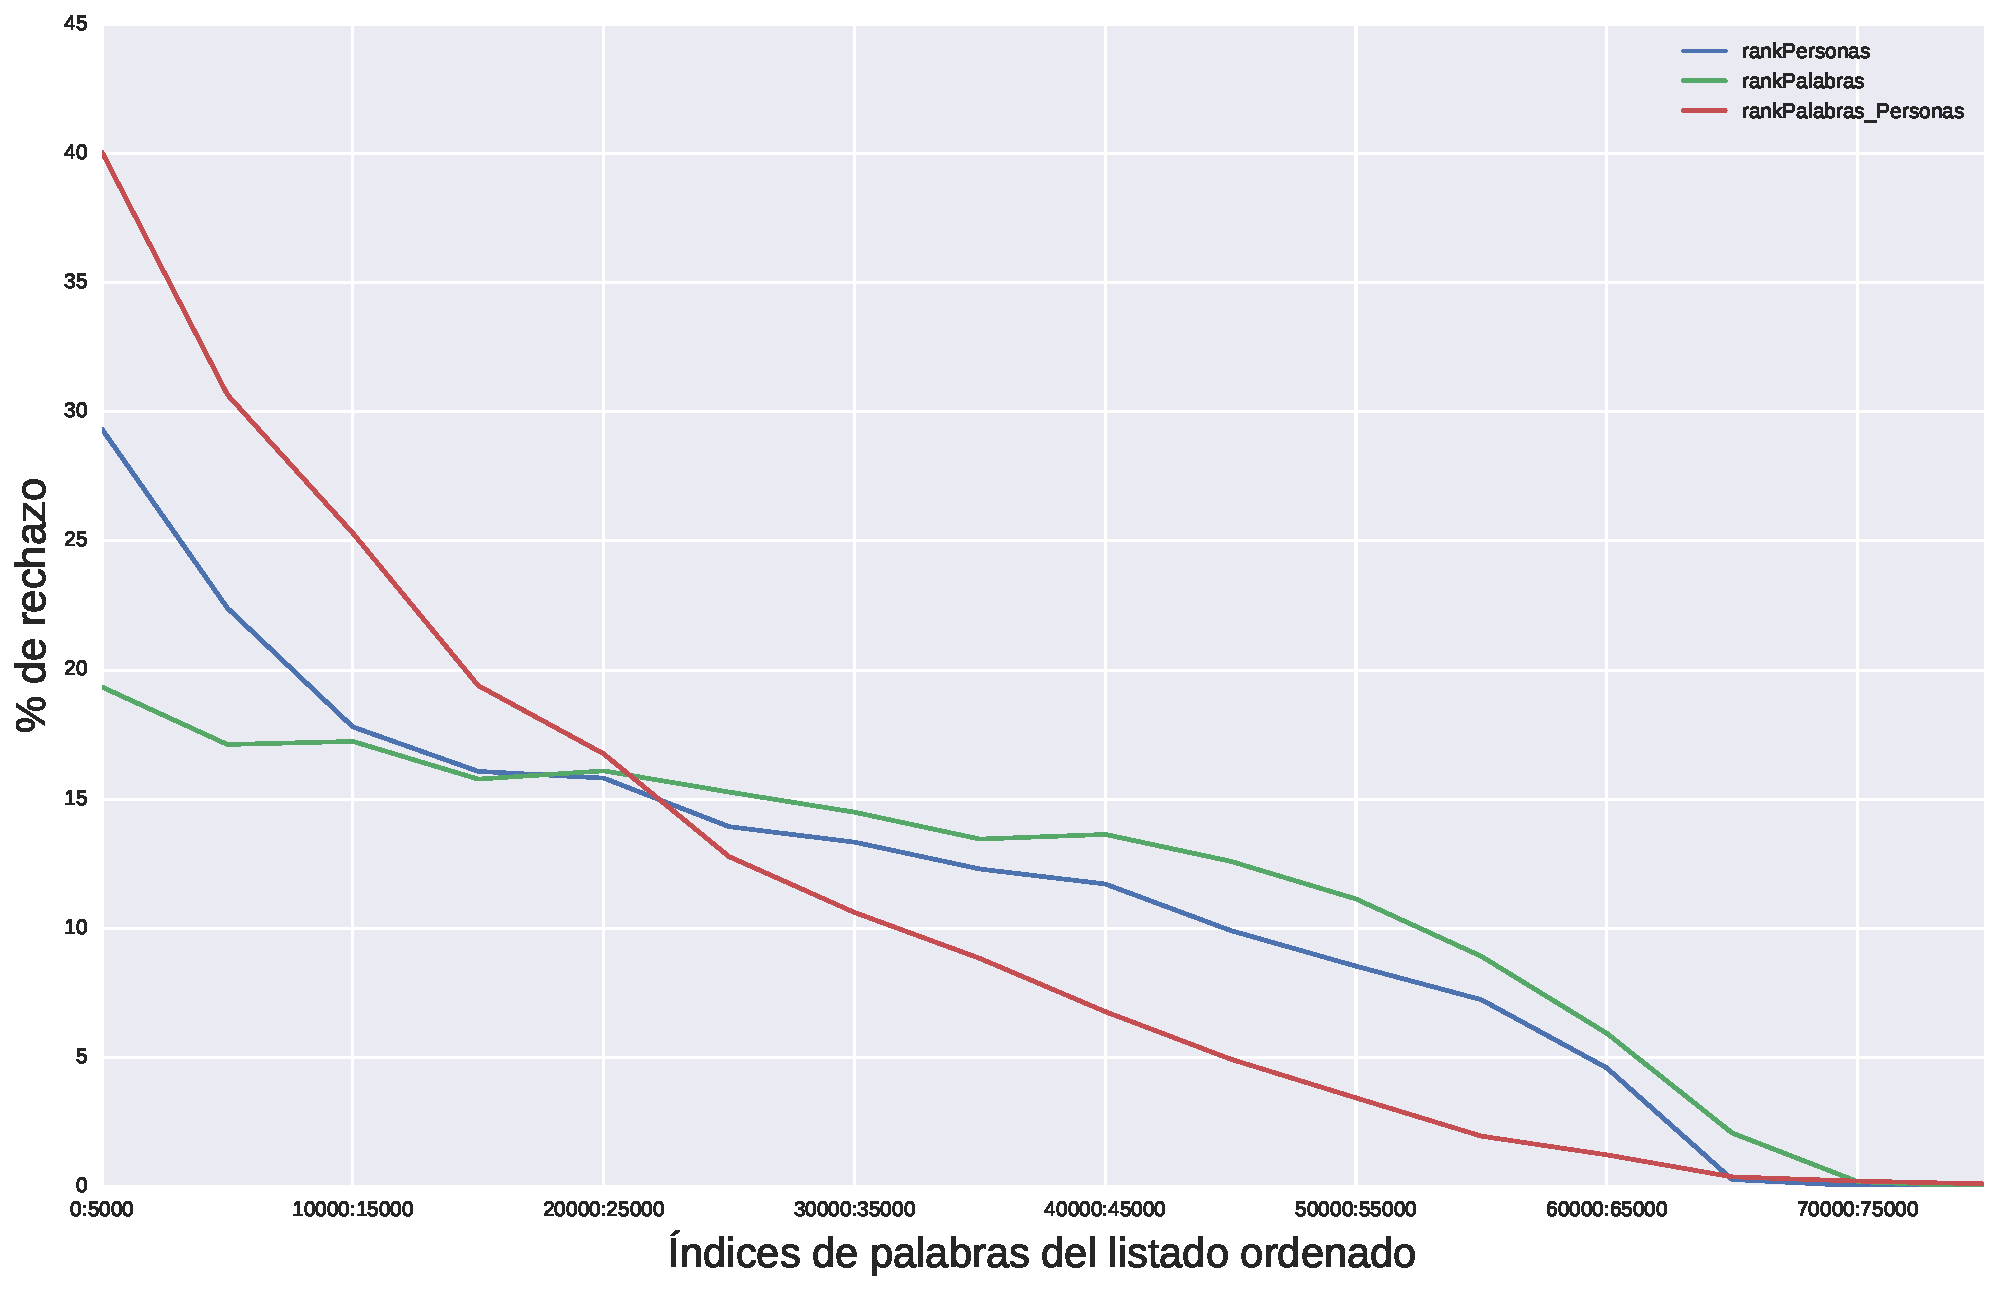
\includegraphics[width=0.6\linewidth]{../src/images/rechazo_metricas.pdf}
            % \label{fig:rechazo_metricas} 
  
  \end{figure}
            
\end{frame}